% !TEX root = ../../main.tex

\section{Résultats numériques des schémas de Lawson approchés}

Dans cette section nous effectuerons une comparaison entre les résultats obtenus la section~\ref{sec:3:num} avec une méthode de Lawson où la résolution de la partie linéaire est exacte mais ne contient pas les équations de Maxwell, et la méthode proposée dans la section~\ref{s3:approx} avec une approximation de la partie linéaire, permettant de prendre en compte plus de termes au sein de celle-ci. L'utilisation de troncatures de la série de Taylor, ou d'approximants de Padé, permet toujours d'effectuer le filtrage de l'équation de Vlasov effectué dans la sous-section~\ref{ssec:3:filtrage}.

La condition initiale est choisie de la même manière que précédemment, c'est-à-dire conformément à~\cite{Holderied:2020} :
$$
  f_h(t=0,z,\vb{v}) = \frac{\rho_h}{(2\pi)^{3/2}\bar{v}_{\|}\bar{v}_\perp^2}\exp( - \frac{v_z^2}{2\bar{v}_{\|}^2} - \frac{\left( v_x^2 + v_y^2 \right)^2}{2\bar{v}_\perp^2} )
$$
avec $z\in[0,\frac{2\pi}{k}]$, $k=2$, $\bar{v}_{\|}=0.2$, $\bar{v}_\perp=0.6$, $\rho_h=0.2$ et $B_x(t=0,z)=\epsilon\sin(kz)$. Les autres inconnues du système $(j_{c,x},j_{c,y},B_y,E_x,E_y)$ sont initialisées à zéro. Le domaine en vitesse est restreint à $\vb{v}\in[-3.6,3.6]\times[-3.6,3.6]\times[-2.4,2.4]$ et on note $N_z$, $N_{v_x}$, $N_{v_y}$, $N_{v_z}$ le nombre de points de discrétisation dans chaque direction.

Dans les diagnostics que nous allons présenter, nous regardons les mêmes quantités, à savoir les énergies magnétiques, électriques et l'énergie cinétique des particules froides, décrites dans les équations~\eqref{eq:3:nrj:me}-\eqref{eq:3:nrj:ce}, ainsi que la préservation de l'énergie totale. Les seuls solveurs que nous étudions dans cette section sont des méthodes de Lawson induites par les méthodes RK(3,3) de Shu-Osher ou RK(4,4), où la partie linéaire sera approchée par une troncature de la série de Taylor ou un approximant de Padé à différents ordres.

\begin{otherlanguage}{english}
Acknowledgment: Experiments presented in this section were carried out using the PlaFRIM experimental testbed, supported by Inria, CNRS (LABRI and IMB), Université de Bordeaux, Bordeaux INP and Conseil Régional d’Aquitaine (see \url{https://www.plafrim.fr/}).
\end{otherlanguage}

\subsection{Comparaison des troncatures à pas de temps constant}

Dans un premier temps nous souhaitons étudier la faisabilité de ne pas résoudre exactement la partie linéaire d'une méthode de Lawson. Pour cela nous conservons la partie linéaire~\eqref{eq:3:LNsmaxwell}, déjà utilisée dans les premiers résultats dans la section~\ref{sec:3:num} et étudions l'impact sur les résultats avec les mêmes paramètres numériques et une méthode d'approximation d'ordre supérieur à la méthode de Lawson LRK(4,4) utilisée, à savoir $T_5$ et $P_{2,2}$. Ces résultats sont observables sur les trois énergies sur la figure~\ref{fig:approx:energies4d}. Les résultats coïncident parfaitement avec les résultats précédents, ce qui permet de confirmer la faisabilité de construire une méthode de Lawson avec une partie linéaire approchée qui contient les équations de Maxwell.

\begin{figure}[h]
  \centering
  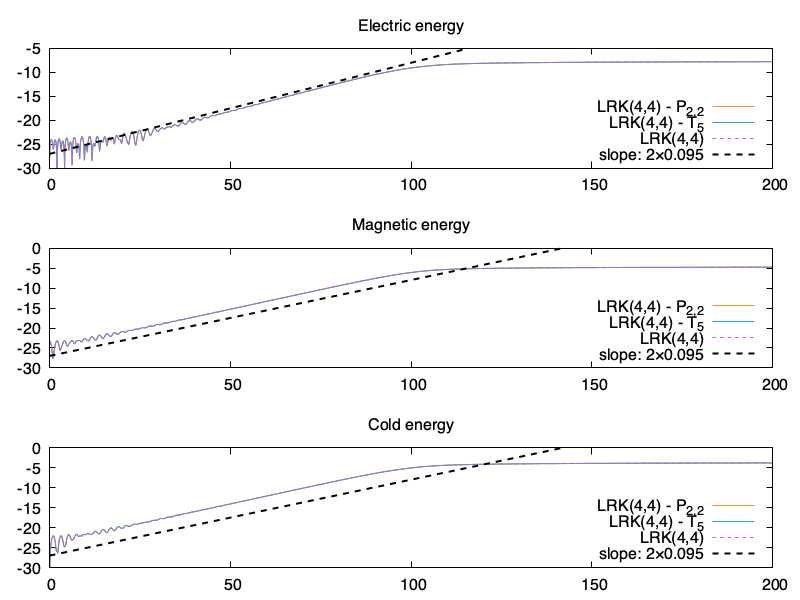
\includegraphics[width=0.9\textwidth]{\localPath/figures/energy_verif.png}
  \caption{Évolution de l'énergie électrique, magnétique et l'énergie cinétique des particules froides définies dans les équations~\ref{eq:3:nrj:me}-\ref{eq:3:nrj:ce}, en échelle semi-$\log$, pour les méthodes de Lawson LRK(4,4) classique, avec troncature de la série de Taylor à l'ordre 5 $T_5$, et approximant de Padé d'ordre $(2,2)$ $P_{2,2}$. $\Delta t = 0.05, N_x=27, N_{v_x}=32, N_{v_y}=32, N_{v_z}=41$.}
  \label{fig:approx:energies4d}
\end{figure}

Sur la figure~\ref{fig:approx:energies:cfl} on teste avec la partie linéaire données par~\eqref{eq:3:LNmaxwell} et étudiée dans la section~\ref{s3:approx}, avec un pas de temps deux fois plus grand que précédemment. On remarque que les résultats sont très similaires. \Josselin{Lancer des runs en limite de CFL (avec Maxwell, prendre le 0.12 donné par la simu DP4(3), et potentiellement une autre un peu plus bas) et comparer avec des résultats sans Maxwell (et voir exploser en temps court dans la phase linéaire), bref comparer Maxwell \emph{inside} et Maxwell \emph{outside}. Donc il reste quelques runs à lancer pour améliorer ça.}

\begin{figure}[h]
  \centering
  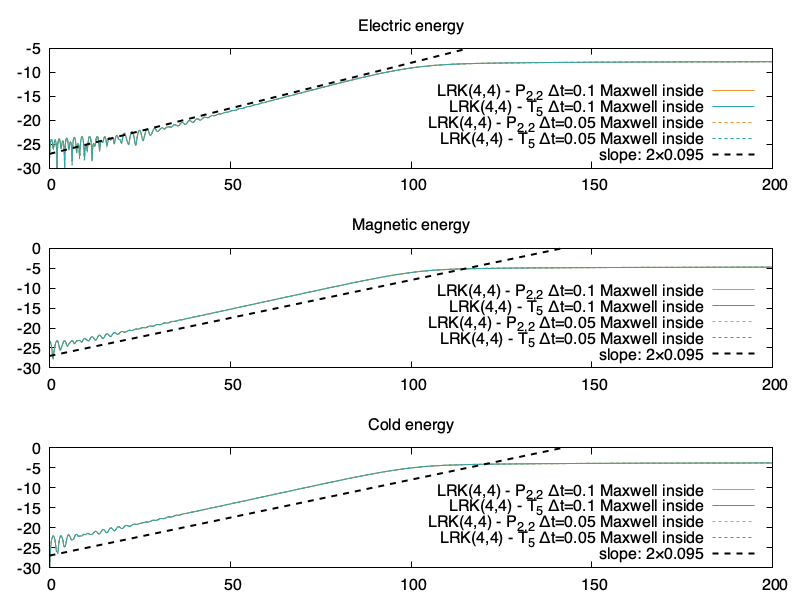
\includegraphics[width=0.9\textwidth]{\localPath/figures/energy_max.png}
  \caption{Évolution de l'énergie électrique, magnétique et l'énergie cinétique des particules froides définies dans les équations~\ref{eq:3:nrj:me}-\ref{eq:3:nrj:ce}, en échelle semi-$\log$, pour les méthodes de Lawson LRK(4,4) classique, avec troncature de la série de Taylor à l'ordre 5 $T_5$, et approximant de Padé d'ordre $(2,2)$ $P_{2,2}$. $\Delta t \in \{0.05,0.1\}, N_x=27, N_{v_x}=32, N_{v_y}=32, N_{v_z}=41$.}
  \label{fig:approx:energies:cfl}
\end{figure}

Nous étudions maintenant pour l'influence sur les résultats de différents approximants de Padé. En particulier nous testons des ordres inférieurs à la méthode de Lawson, ainsi que des approximants de Padé avec des degrés différents pour le numérateur et le dénominateur ($P_{1,2}$ et $P_{2,1}$). On remarque sur la figure~\ref{fig:approx:energies:pade} que l'on a une très bonne correspondance dans les résultats entre les différents approximants de Padé et les résultats précédent ou les relations de dispersions. Il n'y a que le cas où le degré du numérateur est supérieur au dénominateur que le schéma est instable, comme prédit par la théorie. \Josselin{je n'ai encore rien écrit là dessus dans la section~\ref{s3:approx}.}

\begin{figure}[h]
  \centering
  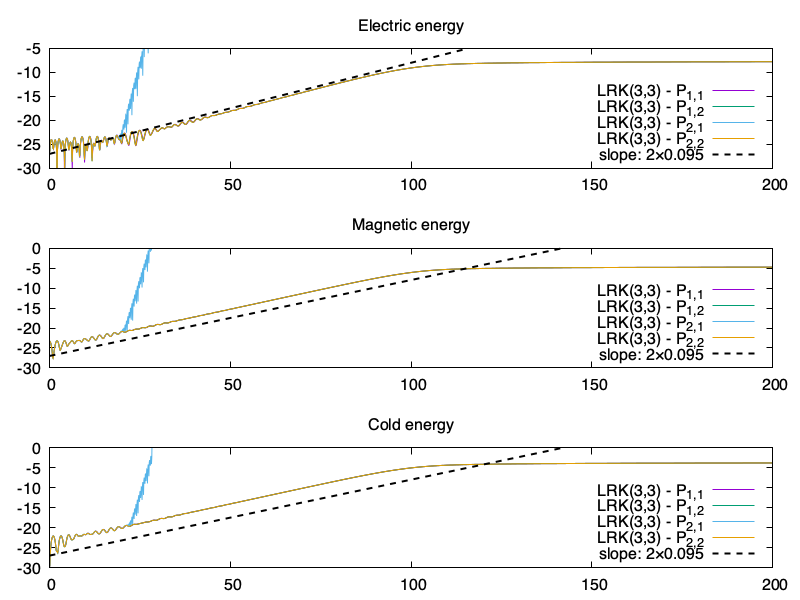
\includegraphics[width=0.9\textwidth]{\localPath/figures/energy_pade.png}
  \caption{Évolution de l'énergie électrique, magnétique et l'énergie cinétique des particules froides définies dans les équations~\ref{eq:3:nrj:me}-\ref{eq:3:nrj:ce}, en échelle semi-$\log$, pour les méthodes de Lawson LRK(3,3) de Shu-Osher, avec différents approximant de Padé d'ordre $(1,1)$, $(1,2)$, $(2,1)$ et $(2,2)$. $\Delta t = 0.1, N_x=27, N_{v_x}=32, N_{v_y}=32, N_{v_z}=41$.}
  \label{fig:approx:energies:pade}
\end{figure}

\subsection{Étude à pas de temps adaptatif}

\begin{figure}[h]
  \centering
  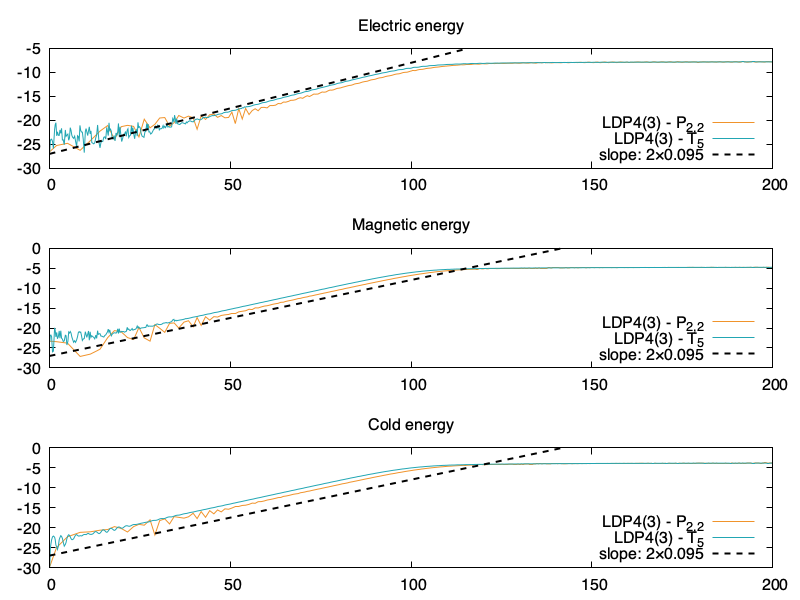
\includegraphics[width=0.9\textwidth]{\localPath/figures/energy_dtn.png}
  \caption{Évolution de l'énergie électrique, magnétique et l'énergie cinétique des particules froides définies dans les équations~\ref{eq:3:nrj:me}-\ref{eq:3:nrj:ce}, en échelle semi-$\log$, pour les méthodes de Lawson LRK(4,4) avec troncature de la série de Taylor à l'ordre 5 $T_5$, et approximant de Padé d'ordre $(2,2)$ $P_{2,2}$. $\Delta t_0 = 0.1, N_x=27, N_{v_x}=32, N_{v_y}=32, N_{v_z}=41$.}
  \label{fig:approx:energies:dtn}
\end{figure}
